






% =========----------	[ Space left here for distraction free mode] ----------==========%









\subsection{Analysis 5: Is there a correlation between spatial attribute score and selected timbral attributes?}

	Correlation coefficients were calculated for each combination of spatial attribute score against timbral attribute score. Most calculations returned weak correlations with $p > 0.05$ other than two timbral attributes specifically when comparing against the 'envelopment' spatial attribute. Figure~\ref{image:corr_env} shows the line of best fit for all timbral attribute scores against the spatial attribute scores for 'envelopment'. The dashed lines indicate a statistically significant correlation as found with the timbral attributes 'Full' and 'Realistic'. The graph indicates that there is a significant positive correlation between the increase in sense of envelopment in the virtual environment with the sense of the virtual environment sounding realistic.

	The data also indicates a negative correlation between participants sense of envelopment and their perception of the timbre sounding 'Full'. The reason as to why this is is not exactly clear. It could be said that participants perception of 'Full' may mean an unnatural abundance of bass frequencies which may sound unrealistic. If this is the case, as we can see from the positive correlation between a sense of envelopment and a sense of the environment sounding realistic, that an unrealistic sounding environment would lead to a decrease in participants sense of envelopment. 

	\textbf{Conclusion}

	The only spatial attribute to show a significant correlation with timbral attribute data is 'Sense of Space' with a positive correlation for a perception of the mix sounding 'Realistic' and a negative correlation for the perception of the mix sounding 'Full'.

	\begin{figure}
		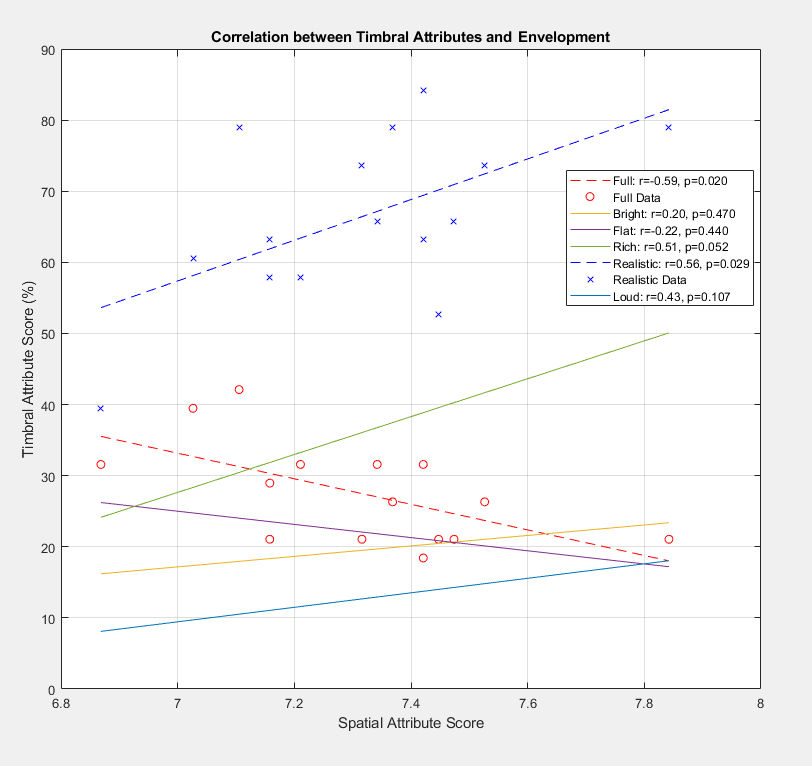
\includegraphics[width=\linewidth]{images/plots/sa_ta_corr_env.PNG}
		\caption{Graph showing correlations between Timbral Attribute and Envelopment scores where dashed lines indicate a statistically significant correlation for which their individual data points have also been plotted.}
		\label{image:corr_env} 
	\end{figure}		
